\section{初始可行基}
\label{sec:simplex-initial-basis}

上一节的算法要从一个可行基出发，而工厂例子里松弛变量恰好提供了一个。本节解决没有现成可行基时怎么办。

给工厂加一个合同要求：两种产品合计至少交付$2$单位，即$x_1+x_2\geq2$。这个不等式要减去一个非负的剩余变量$x_6$才能化成等式，标准型的第四行是
\begin{equation}
 x_1+x_2-x_6=2.
 \label{eq:simplex-order-row}
\end{equation}
若仍取松弛变量和剩余变量组成基，第四行给出$x_6=-2<0$，不可行。这对应图~\ref{fig:simplex-two-phase-path}中的原点：什么都不生产，合同就违约了，原点已不在可行域内。等式约束的情形更直接，它没有松弛变量可用。

\paragraph{人工变量}
解决办法是暂时允许约束被违反，并给违反量记账。把各行乘以适当的符号使$\bm{b}\geq\bm{0}$，对缺少现成基列的行，引入非负的\term{人工变量}（artificial variable）$\bm{v}$，得到扩大的约束
\begin{equation}
 \bm{A}\bm{x}+\bm{v}=\bm{b},\qquad \bm{x}\geq\bm{0},\quad \bm{v}\geq\bm{0}.
 \label{eq:simplex-artificial-system}
\end{equation}
为叙述简单，这里写成每行都加人工变量；已有松弛变量可作基列的行不必加，例中只有第四行需要。

这个系统立刻有可行基：$\bm{x}=\bm{0}$，$\bm{v}=\bm{b}$。但要分清，它是扩大问题的可行基，不是原问题的：只要某个$v_i>0$，对应的原约束就没有被满足。$\bm{v}$像一笔临时垫付的账，只有全部还清，得到的点才是原问题的可行点。

例中把人工变量记作$x_7$，扩大后的约束有四行七列：
\[
 \begin{bmatrix}
 1&2&1&0&0&0&0\\
 2&1&0&1&0&0&0\\
 0&1&0&0&1&0&0\\
 1&1&0&0&0&-1&1
 \end{bmatrix}\bm{x}
 =\begin{bmatrix}8\\10\\3\\2\end{bmatrix}.
\]
起始基$(3,4,5,7)$的基矩阵是单位矩阵，$x_7=2$就是合同的缺口。两阶段法和大M法用两种方式把这笔账还清。

\subsection{两阶段法}
\label{sec:simplex-two-phase}

\paragraph{主要思想}
\term{两阶段法}（two-phase method）把“还清账”和“优化目标”分开。第一阶段暂时不管原目标，只最小化人工变量之和：
\begin{equation}
 \min_{\bm{x},\bm{v}}\ \phi=\bm{1}^\top\bm{v}
 \quad\text{s.t.}\quad
 \bm{A}\bm{x}+\bm{v}=\bm{b},\quad\bm{x}\geq\bm{0},\quad\bm{v}\geq\bm{0}.
 \label{eq:simplex-phase-one}
\end{equation}
这个问题有现成的可行基，目标又以$0$为下界，所以单纯形法不会遇到无界，一定有最优值$\phi^\star\geq0$。它回答了可行性问题。

\begin{theorem}[第一阶段的结论]
 \label{thm:simplex-phase-one}
 原问题$\bm{A}\bm{x}=\bm{b}$，$\bm{x}\geq\bm{0}$可行，当且仅当问题~\eqref{eq:simplex-phase-one}的最优值$\phi^\star=0$。若$\phi^\star>0$，设$\bm{y}$是第一阶段最优基的对偶候选，则
 \begin{equation}
  \bm{A}^\top\bm{y}\leq\bm{0},\qquad \bm{b}^\top\bm{y}=\phi^\star>0,
  \label{eq:simplex-farkas-certificate}
 \end{equation}
 这个$\bm{y}$就是原问题不可行的证书。
\end{theorem}

\begin{proof}
 若原问题有可行点$\bm{x}$，则$(\bm{x},\bm{0})$对问题~\eqref{eq:simplex-phase-one}可行，目标为零，又因$\phi\geq0$，所以$\phi^\star=0$。反过来，$\phi^\star=0$时最优解满足$\bm{v}=\bm{0}$，它的$\bm{x}$部分满足$\bm{A}\bm{x}=\bm{b}$，$\bm{x}\geq\bm{0}$。

 设$\phi^\star>0$。第一阶段的目标系数在$\bm{x}$上是零，于是最优性条件$s_j=0-\bm{a}_j^\top\bm{y}\geq0$说明$\bm{A}^\top\bm{y}\leq\bm{0}$。由定理~\ref{thm:simplex-optimality}，两边目标值相等，即$\bm{b}^\top\bm{y}=\phi^\star$。若存在$\bm{x}\geq\bm{0}$满足$\bm{A}\bm{x}=\bm{b}$，就有
 \[
  0<\bm{b}^\top\bm{y}=\bm{x}^\top\bm{A}^\top\bm{y}\leq0,
 \]
 矛盾，这说明$\bm{y}$确实证明了不可行。
\end{proof}

\paragraph{变量}
第一阶段沿用第~\ref{sec:simplex-basis-exchange}节的全部变量，只是下标范围包括人工变量，目标向量换成在$\bm{x}$上为零、在$\bm{v}$上为一的$\bm{g}$。第二阶段回到原来的$\bm{c}$，并去掉人工变量对应的列。

\paragraph{初始化}
第一阶段从人工变量和可用的松弛变量组成的基出发。例中
\[
 B^{(0)}=(3,4,5,7),\qquad \bm{x}_B^{(0)}=(8,10,3,2)^\top,\qquad \phi=2.
\]

\needspace{6\baselineskip}
\paragraph{每轮更新}
两个阶段的每轮计算都与第~\ref{sec:simplex-basis-exchange}节相同，区别只在目标向量和两阶段之间的衔接。
\begin{enumerate}
 \item 第一阶段按$\bm{g}$运行单纯形法，直到约化成本全部非负。例中第$0$轮的对偶候选和约化成本为
 \[
  \bm{y}^{(0)}=(0,0,0,1)^\top,\qquad s_1=-1,\quad s_2=-1,\quad s_6=1.
 \]
 $s_1,s_2$并列最负，取下标小的$x_1$入基。它的表示和比值为
 \[
  \bm{u}^{(0)}=(1,2,0,1)^\top,\qquad
  \frac{8}{1}=8,\quad \frac{10}{2}=5,\quad \frac{2}{1}=2.
 \]
 于是$\alpha^{(0)}=2$，$x_7$出基，更新后
 \[
  B^{(1)}=(3,4,5,1),\qquad \bm{x}_B^{(1)}=(6,6,3,2)^\top,\qquad\phi=0.
 \]
 第$1$轮人工变量已经出基，$\bm{y}^{(1)}=\bm{0}$，所有$s_j\geq0$，第一阶段结束，得到$\phi^\star=0$和原问题的顶点$(2,0)$。
 \item 判断$\phi^\star$。若$\phi^\star>0$，按定理~\ref{thm:simplex-phase-one}报告不可行并给出$\bm{y}$。例中$\phi^\star=0$，继续。
 \item 处理仍在基中的人工变量（做法见下文）。例中人工变量已经出基，无需处理。
 \item 第二阶段用基$B^{(1)}$和原目标$\bm{c}$继续运行单纯形法。例中三轮的数据如下。
\end{enumerate}

第二阶段第$0$轮，基是$(3,4,5,1)$，$f=-8$。对偶候选和约化成本是
\[
 \bm{y}=(0,0,0,-4)^\top,\qquad s_2=-1,\qquad s_6=-4.
\]
$s_6$最负，$x_6$入基，意味着多交付一些。表示向量和有效比值是
\[
 \bm{u}=(1,2,0,-1)^\top,\qquad \frac{6}{1}=6,\qquad \frac{6}{2}=3.
\]
于是$\alpha=3$，$x_4$出基，更新后
\[
 B=(3,6,5,1),\qquad \bm{x}_B=(3,3,3,5)^\top,\qquad f=-20.
\]

第二阶段第$1$轮，点在$(5,0)$。对偶候选和约化成本是
\[
 \bm{y}=(0,-2,0,0)^\top,\qquad s_2=-3,\qquad s_4=2.
\]
$x_2$入基。表示向量和三个有效比值是
\[
 \bm{u}=\Bigl(\frac32,-\frac12,1,\frac12\Bigr)^\top,\qquad
 \frac{3}{3/2}=2,\quad \frac{3}{1}=3,\quad \frac{5}{1/2}=10.
\]
于是$\alpha=2$，$x_3$出基，更新后
\[
 B=(2,6,5,1),\qquad \bm{x}_B=(2,4,1,4)^\top,\qquad f=-26.
\]

第二阶段第$2$轮，对偶候选和约化成本是
\[
 \bm{y}=(-2,-1,0,0)^\top,\qquad s_3=2,\qquad s_4=1.
\]
全部非负，算法停止。

\paragraph{最终得到}
最优解仍是$(x_1,x_2)=(4,2)$，$p^\star=-26$，此时$x_6=4$表示比合同多交付了$4$。合同约束在最优点不活动，对偶分量$y_4=0$，加上它并不改变答案。图~\ref{fig:simplex-two-phase-path}画出了两个阶段的路径。

\begin{BookInlineFigure}
 \centering
 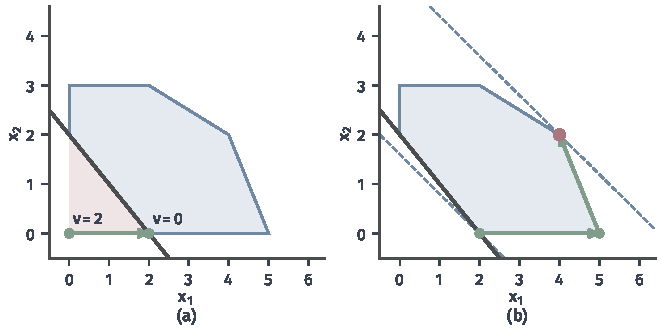
\includegraphics[width=112mm]{figures/05-optimization/01-linear-programming/matplotlib/simplex-two-phase-path/figure.pdf}
 \caption{两阶段法的路径。深灰粗线是合同约束$x_1+x_2=2$，浅蓝是原问题的可行域，它不含原点。(a)~第一阶段：从不可行的原点出发（红色浅底是违约区），沿$x_1$轴走到人工变量$v=x_7$降为零的点。(b)~第二阶段：从$(2,0)$出发，用原目标走到红色的最优点，蓝色虚线是利润$8$和$26$的等值线。}
 \label{fig:simplex-two-phase-path}
\end{BookInlineFigure}

\paragraph{第一阶段判定不可行}
把合同改成$x_1+x_2\geq7$。第一阶段从$\phi=7$开始，三轮的基和人工变量值为
\[
 \begin{aligned}
 B^{(0)}&=(3,4,5,7),& x_7&=7,\\
 B^{(1)}&=(3,1,5,7),& x_7&=2,\\
 B^{(2)}&=(2,1,5,7),& x_7&=1.
 \end{aligned}
\]
第$2$轮的对偶候选和约化成本是
\[
 \bm{y}=\Bigl(-\frac13,-\frac13,0,1\Bigr)^\top,\qquad
 s_3=\frac13,\quad s_4=\frac13,\quad s_6=1.
\]
全部非负而$\phi^\star=1>0$，原问题不可行。

证书$\bm{y}$可以翻译成一句平常的话。原料和工时两个约束各乘$\frac13$相加，得到$x_1+x_2\leq6$，这与$x_1+x_2\geq7$矛盾，差额正好是$\phi^\star=1$。图~\ref{fig:simplex-phase-one-infeasible}中，第一阶段把点推到离合同线最近的顶点，停在那里，仍差$1$。

\begin{BookInlineFigure}
 \centering
 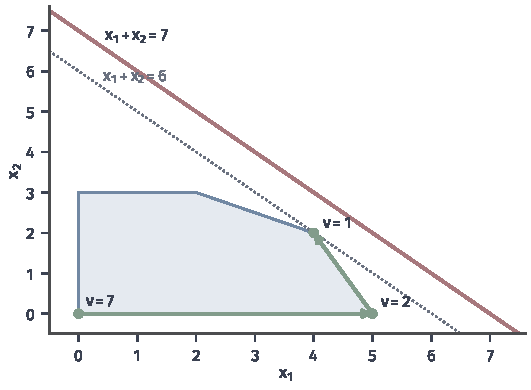
\includegraphics[width=90mm]{figures/05-optimization/01-linear-programming/matplotlib/simplex-phase-one-infeasible/figure.pdf}
 \caption{合同要求提高到$x_1+x_2\geq7$时的第一阶段。红线是合同边界，点线$x_1+x_2=6$是资源约束组合出的上限，两者之间没有可行点。绿色路径沿资源多边形的边界推进，人工变量$v$依次取$7,2,1$，在第一阶段最优点停在$v=1$。}
 \label{fig:simplex-phase-one-infeasible}
\end{BookInlineFigure}

\paragraph{基中残留的人工变量}
$\phi^\star=0$时，人工变量的值全为零，但可能有个别人工变量仍在基中，取值为零。第二阶段不能直接开始，否则人工变量可能在后续换基中重新变正。设它位于基的第$r$个位置，定义该行的系数
\begin{equation}
 \bm{\rho}=\bm{A}_B^{-\top}\bm{e}_r,\qquad \bar{a}_{r,j}=\bm{\rho}^\top\bm{a}_j,
 \label{eq:simplex-row-coefficients}
\end{equation}
其中$\bm{e}_r$是第$r$个坐标向量，$\bar{a}_{r,j}$就是把$\bm{a}_j$用基表示时第$r$个分量。分两种情况处理。

\begin{itemize}
 \item 存在原变量$x_j$（$j\in N$）使$\bar{a}_{r,j}\neq0$。把$x_j$换入第$r$个位置。由于该位置的值是零，步长为零，其他变量不变，符号不必为正。
 \item 对所有原变量都有$\bar{a}_{r,j}=0$。此时$\bm{\rho}^\top\bm{A}=\bm{0}^\top$，$\bm{\rho}\neq\bm{0}$，说明这一行是其余行的线性组合，是冗余等式，可以连同该人工变量一起删去。
\end{itemize}

第二种情况也说明，第~\ref{chap:linear-programming}章假定$\bm{A}$满行秩并不需要预先检查，第一阶段顺带就发现了冗余行。下面的例子展示两种情况。

\begin{example}[换出与删行]
 \label{ex:simplex-residual-artificial}
 考虑约束$x_1+x_2+x_3=2$，$2x_1+\omega(x_2+x_3)=4$，$\bm{x}\geq\bm{0}$，其中$\omega$取$1$或$2$，人工变量是$x_4,x_5$。从基$(4,5)$出发，$x_1$的约化成本最负。比值都是$2$，并列时取下标小的$x_4$出基，得到基$(1,5)$和
 \[
  \bm{x}_B=(2,0)^\top,\qquad \phi=0,\qquad\bm{\rho}=(-2,1)^\top.
 \]
 $x_5$在基中取零。

 取$\omega=1$时，系数是$\bar{a}_{2,2}=\bar{a}_{2,3}=-1\neq0$，把$x_2$换入第$2$个位置，步长为零，基变为$(1,2)$。

 取$\omega=2$时，系数是$\bar{a}_{2,2}=\bar{a}_{2,3}=0$。第二行正是第一行的$2$倍，删去第二行和$x_5$，基变为$(1)$。
\end{example}

图~\ref{fig:simplex-phase-flow}把两阶段法的分支整理在一起。

\begin{BookInlineFigure}
 \centering
 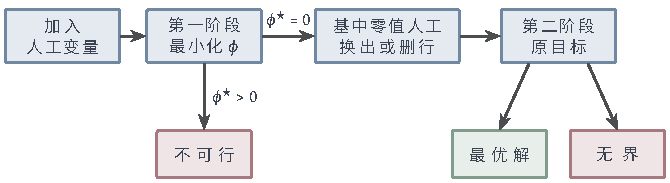
\includegraphics[width=112mm]{figures/05-optimization/01-linear-programming/tikz/simplex-phase-flow/figure.pdf}
 \caption{两阶段法的流程。第一阶段的最优值$\phi^\star$决定是否继续；基中取零的人工变量换出或连同冗余行删去后，第二阶段以原目标运行，以最优解或无界方向结束。红框是给出证书的否定结果，绿框是得到最优解。}
 \label{fig:simplex-phase-flow}
\end{BookInlineFigure}

\subsection{大M法}
\label{sec:simplex-big-m}

\paragraph{主要思想}
\term{大M法}（big-M method）把两个阶段合成一个问题，在目标中给人工变量定一个极高的单价：
\begin{equation}
 \min_{\bm{x},\bm{v}}\ \bm{c}^\top\bm{x}+M\,\bm{1}^\top\bm{v}
 \quad\text{s.t.}\quad
 \bm{A}\bm{x}+\bm{v}=\bm{b},\quad\bm{x}\geq\bm{0},\quad\bm{v}\geq\bm{0}.
 \label{eq:simplex-big-m}
\end{equation}
把$M$当作一个比任何数都大的符号来计算，约化成本就是形如$\beta+\gamma M$的式子，比较大小时先比$\gamma$，再比$\beta$。这样，只要还能减少人工变量，算法就不会先去改善原目标，排除人工变量自动享有优先权。

例中第$0$轮的对偶候选和约化成本是
\[
 \bm{y}=(0,0,0,M)^\top,\quad s_1=-4-M,\quad s_2=-5-M,\quad s_6=M.
\]
$s_1,s_2$里$M$的系数相同，再比常数项，$s_2$更负，$x_2$入基。此后各轮的数据在表~\ref{tab:simplex-big-m-rounds}中，路径见图~\ref{fig:simplex-big-m}(a)。第$0$轮换基后人工变量已经出基，接下来就是用原目标继续。

\begin{BookInlineTable}
 \centering
 \begin{tabular}{cccc}
  \toprule
  $t$ & $B^{(t)}$ & $(x_1,x_2)$ & 负的约化成本（入基）\\
  \midrule
  $0$ & $(3,4,5,7)$ & $(0,0)$ & $s_2=-5-M$，$s_1=-4-M$\\
  $1$ & $(3,4,5,2)$ & $(0,2)$ & $s_6=-5$\\
  $2$ & $(3,4,6,2)$ & $(0,3)$ & $s_1=-4$\\
  $3$ & $(1,4,6,2)$ & $(2,3)$ & $s_5=-3$\\
  $4$ & $(1,5,6,2)$ & $(4,2)$ & 无，停止\\
  \bottomrule
 \end{tabular}
 \caption{符号化大M法的各轮数据。}
 \label{tab:simplex-big-m-rounds}
\end{BookInlineTable}

\paragraph{有限的$M$要多大}
实际计算若取一个具体的数$M$，就必须问它够不够大。下面的定理给出精确的条件。

\begin{theorem}[有限惩罚的充分条件]
 \label{thm:simplex-finite-penalty}
 设标准型~\eqref{eq:simplex-standard-form}有最优解，最优值为$p^\star$，$\bm{y}^\star$是一个对偶最优解。若
 \begin{equation}
  M>\max_i\,y_i^\star,
  \label{eq:simplex-big-m-threshold}
 \end{equation}
 其中$i$取遍带人工变量的行，则问题~\eqref{eq:simplex-big-m}的最优值等于$p^\star$，并且它的每个最优解都满足$\bm{v}=\bm{0}$，其$\bm{x}$部分是原问题的最优解。
\end{theorem}

\begin{proof}
 为简洁起见设每行都有人工变量，其余情形只需令相应$v_i=0$。任取问题~\eqref{eq:simplex-big-m}的可行点$(\bm{x},\bm{v})$，记对偶松弛为$\bm{s}^\star\geq\bm{0}$，它满足$\bm{c}=\bm{s}^\star+\bm{A}^\top\bm{y}^\star$。把$\bm{c}$代换掉，并用$\bm{A}\bm{x}=\bm{b}-\bm{v}$，得到
 \[
  \bm{c}^\top\bm{x}
  =(\bm{s}^\star)^\top\bm{x}+(\bm{y}^\star)^\top\bm{A}\bm{x}
  \geq(\bm{y}^\star)^\top\bm{b}-(\bm{y}^\star)^\top\bm{v}.
 \]
 由强对偶，$\bm{b}^\top\bm{y}^\star=p^\star$，于是两边加上$M\bm{1}^\top\bm{v}$后，
 \[
  \bm{c}^\top\bm{x}+M\bm{1}^\top\bm{v}
  \geq p^\star+\sum_i(M-y_i^\star)v_i\geq p^\star.
 \]
 原问题的最优解配上$\bm{v}=\bm{0}$可行且取到$p^\star$，所以最优值是$p^\star$。若某个最优解有$v_i>0$，由式~\eqref{eq:simplex-big-m-threshold}上面最后一个不等号严格成立，与最优值为$p^\star$矛盾，所以$\bm{v}=\bm{0}$。此时$\bm{x}$可行且目标为$p^\star$，是原问题的最优解。
\end{proof}

门槛是对偶价格，这很合理：$y_i^\star$是放松第$i$条约束一单位时目标能下降多少，$M$是违反一单位约束要付的罚款。罚款高过这个收益，违约才不划算。

这个门槛取决于事先并不知道的$\bm{y}^\star$。把工厂的目标换成最小化成本$2x_1+3x_2$，合同约束就变成活动约束，最优解是$(2,0)$，对偶分量$y_4^\star=2$。图~\ref{fig:simplex-big-m}(b)对每个$M$精确求解，$M<2$时最优解干脆不生产，留着$v=2$付罚款，$M>2$时才回到真正的解。

\begin{BookInlineFigure}
 \centering
 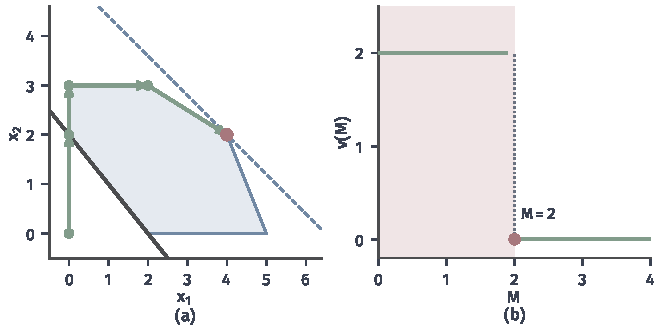
\includegraphics[width=112mm]{figures/05-optimization/01-linear-programming/matplotlib/simplex-big-m/figure.pdf}
 \caption{大M法。(a)~符号化大M在资源配置问题上的路径（绿色），第一步消去人工变量到达$(0,2)$，其后沿边界到最优点。(b)~目标$2x_1+3x_2+Mv$在不同有限$M$下的最优人工变量值$v(M)$：红色浅底的$M<2$区间内罚款不足，解停留在$v=2$；$M=2$时两种解并列（点线）；$M>2$时$v=0$。}
 \label{fig:simplex-big-m}
\end{BookInlineFigure}

$M$也不能随意取大。在双精度浮点数中，$10^{17}$附近相邻两个可表示数相差$16$，于是
\[
 -4-10^{17}\quad\text{和}\quad-5-10^{17}
\]
舍入后是同一个数，$c_1=-4$与$c_2=-5$的差别被抹掉，定价失去依据。系数相差过于悬殊还会使基矩阵病态。所以有限$M$不能靠“取一个很大的常数”得到保证；另外，若某个有限$M$的解有$v\neq\bm{0}$，也分不清是$M$不够大还是原问题不可行。

表~\ref{tab:simplex-two-phase-vs-big-m}对照了两种做法。

\begin{BookInlineTable}
 \centering
 \begin{tabular}{lll}
  \toprule
  & 两阶段法 & 大M法\\
  \midrule
  目标 & 先最小化$\bm{1}^\top\bm{v}$，再用$\bm{c}$ & 同时用$\bm{c}+M$惩罚\\
  不可行判定 & $\phi^\star>0$ & 符号化时$\bm{v}$不能消去\\
  参数 & 无 & 需要符号或足够大的$M$\\
  数值风险 & 无额外系数 & $M$过大使尺度恶化\\
  \bottomrule
 \end{tabular}
 \caption{两阶段法与大M法的对照。}
 \label{tab:simplex-two-phase-vs-big-m}
\end{BookInlineTable}
